\documentclass[a4paper,12pt]{article}
\usepackage{makeidx}
\usepackage[T1]{fontenc}
\usepackage{amsmath,amscd,amsthm}
\usepackage{amssymb}
\usepackage{tabularx}
\usepackage{amssymb,eucal,bezier,graphicx}
\usepackage{times,amssymb}
\usepackage[ansinew]{inputenc}
\usepackage{multicol}
\usepackage{hyperref}
\usepackage{multicol}
\usepackage{verbatim}
\usepackage{tikz-cd}
\usetikzlibrary{graphs}
\usetikzlibrary{arrows.meta}

\newtheorem{thm}{Theorem}[section]
\newtheorem{cor}[thm]{Collorary}
\newtheorem{lemma}[thm]{Lemma}
\newtheorem{prop}[thm]{Proposition}
\newtheorem{prob}[thm]{Problema}
\newtheorem{defi}[thm]{Definition}
\newtheorem{conj}[thm]{Conjecture}
\newtheorem{nota}[thm]{Note}
\newtheorem{ejem}[thm]{Example}

\newtheorem{demo}[thm]{Proof}
\providecommand{\gabs}[1]{\left|{#1}\right|}
\begin{document}

%%Los tres siguientes comandos estaban inicialmente desinsertados, pero no funcionaban en concordancia en el texto

\renewcommand{\figurename}{Figure}

\renewcommand\thefigure{\arabic{section}.\arabic{figure}} 

\numberwithin{figure}{section} 
%\renewcommand{\thebibliography}{References}

%\addto\captionsspanish{%
%\def\bibname{References}%
%}



\begin{center} {\large \bf Estudio de la Conjetura de Gilbreath}
\end{center}


\begin{center}
{\bf Eleazar Duarte Aponte, Rafael Gonz�lez L�pez,\\
Roc�o Palacios Cantillo, Luis Palma Blanco,\\
Diego Pedraza L�pez}
\end{center}

\begin{center}
\small{ Teor�a Anal�tica de N�meros \\
\small Universidad de Sevilla. }
\end{center}

\vspace{0.4cm}

\begin{center}
{\bf Abstract}

\end{center}

\begin{quotation}
\noindent En este trabajo vamos a TAL TAL TAL
\end{quotation}

\vspace{0.1cm}



\section*{Introducci�n}


%to continue the research on a
%new mathematical topic emerged not long ago, the {\em evolution
%algebras}, to obtain new results from those already obtained by
%Tian (see \cite{book, Petr}) and two of the authors in two
%previous works (\cite{AMC} and \cite{NRV}), relying on tools in
%principle away from these algebras as
% directed graphs and Markov chains are.
%
%\vspace{0.1cm}
%
%The motivation to deal with evolution algebras is the following. At present,
%the study of these algebras is very booming, due to the numerous connections
%between them and many other branches of Mathematics, such as Graph Theory,
%Group Theory, Markov Processes, Dynamic Systems and Theory of Knots,
%among others. Furthermore, they are also related to other sciences, including
%Biology, since non-Mendelian genetics is precisely which originated them. In fact,
%Tian already indicated in Chapter 2 of \cite{book} the relationship between evolution algebras
%evolution and Markov chains.
%
%\vspace{0.1cm}
%
%For this study we have used in this paper certain objects of Discrete Mathematics,
%particularly directed graphs, thus linking three branches of the
%Mathematic which at first would appear to have no connection: algebras of evolution
%Theory, Graph Theory and Markov chains, so that the attainment of new
%properties of each of them allows to achieve certain advances in the study of the
%others.
%
%\vspace{0.1cm}
%
%The relationship among these three branches is based on the direct and reverse representation
%of each Markov chain by an evolution algebra and the one  of the latter by
%a certain graph, so that the study of the properties of each of
%these objects allows us its subsequent translation to the language of the other two. This
%research, which could be considered novel, was already somehow used by Tian himself
%in Chapter 6 of \cite{book}.
%
%\vspace{0.1cm}
%
%Recently, several  works regarding the use of graphs for studying  evolution algebras have appeared in the literature (see \cite{AMC}, \cite{NRV}, \cite{cabrera} and \cite{elduque}, for instance). With the results collected in this paper we  present some progress in the link between Markov chains and evolution algebras. We think that  the properties and technics of Markov chains would be useful in the study  of evolution algebras.
%
%\vspace{0.1cm}
%
%The structure of this paper is as follows: Section 1 is devoted to recall some preliminaries on evolution algebras,
%Graph Theory and Markov chains which will be used throughout
%the paper. In Section 2, in which the main results of the paper are shown, we deal with the associations between pairs of these three types of objects.


\section{Preliminaries}

In this section we recall some basic concepts related to evolution
algebras and Graph Theory, to be used in this paper. We also deal
with the links between them. For a more general overview of these
two topics, references \cite {book, Petr} for the first and \cite
{bollo, harary} for the second, among others, are available. In
this paper, all evolution algebras will be considered finite.

\subsection{Preliminaries on Evolution algebras}

Evolution algebras, which  were firstly introduced  by J. P. Tian, and then jointly presented with Vojtechovsky in 2006 \cite{Petr}, and later appeared as a book by Tian in 2008 \cite{book}, are those algebras in which the relationships between their generators $V=\{e_1, \ldots, e_n\}$ are given by
$$
\left\{
\begin{array}{l}
e_i  \cdot e_j = 0, \quad  i \neq j,  \quad 1 \leq i, j \leq n, \\
e_i^2 =e_i  \cdot e_i = \displaystyle \sum_{j = 1}^n a_{ji} \, e_j, \quad  1 \leq i \leq n.
\end{array}
\right.
$$
where $a_{ji} \in K$ and $K$  is a field.

\vspace{0.1cm}

If $E$ is an evolution algebra over a field $K$  with a generator set $V=\{e_i \mid i \in \Lambda\}$, the  linear map $L: E \to E$ $\mid L(e_i) = e^2_i =
 \sum_j a_{ji} e_j$, for all $i \in \Lambda$ is called the {\em evolution operator} of $E$, the coefficients $a_{ji}$ are the {\em structure constants of $E$ relative to } $V$ and the matrix $M_V:=(a_{ji})$ is said to be the {\em structure matrix of $E$ relative to $V$.}

\vspace{0.1cm}

A particular subclass of evolution algebras are the graphicable algebras, also introduced by Tian in \cite{book}. An {\em $n$-dimensional graphicable algebra} is a commutative, non associative algebra, with a set of generators $V = \{e_1, e_2, \dots, e_n \} $ endowed with relations
$$\left\{
\begin{array}{l}
e_i \cdot e_j = 0, \quad i \neq j, \quad 1 \leq i, j \leq n, \\
e_i^2 = \displaystyle \sum_{e_j \subseteq V_i}  e_j, \quad 1 \leq i \leq n. \\
\end{array}
\right.
\newline
$$

where $V_i$ is a subset of $V$.

\vspace{0.1cm}

 \noindent Thus, it is obvious that a graphicable algebra is an evolution algebra, although the converse is not true in general.

\vspace{0.1cm}

An {\em evolution subalgebra} of an evolution algebra spanned by $\{e_1,...,e_n\}$ is a subalgebra that is spanned by $\{e_i: i \in \Lambda \},$ for some subset $\Lambda$ of $\{1, \ldots, n\}.$

\vspace{0.1cm}

Let $E$ be an evolution algebra and $I$ be an evolution subalgebra of $E$. It is said that
$I$ is an {\em evolution ideal} of $E$ if $E\cdot I\subseteq I$. Note that this definition implies that every evolution subalgebra is an evolution ideal.

\vspace{0.1cm}

An evolution algebra $E$ is called {\em simple} if it has not ideals different from $0$ and $E$, and it is called {\em irreducible}
it it has no proper subalgebra.

\vspace{0.1cm}

The following definition is given by Tian in \cite{book}: Let $E$ be an evolution algebra and $\{e_1,e_2,...e_n\}$ a set of generators.
It is said that $e_i$ {\em appears} in $x\in E$ if the coefficient $\alpha_i \in K$ is different from $0$ in the expression
$x= \sum_{j=1}^n \alpha_j e_j$. If $e_i$ appears in $x$, it is denoted by $e_i\prec x$.

\vspace{0.1cm}

\subsection{Preliminaries on Graph Theory}


Moving on now to Graph Theory, the most basic concepts, as simple
graph, directed edge, vertex, adjacency and incidence, adjacency
matrix, subgraph and walk between two vertices of a graph are
assumed to be known (\cite {harary} can be consulted for details).

\vspace{0.1cm}

A {\em weighted directed graph} $G=(V(G),E(G))$ is a pair formed by the set of vertices $V(G)$ of the graph, the set of directed edges $E(G)$ of the graph
and a function $\omega$ defined over the edges, $\omega: E(G) \to \mathbb{R}$. The image of the function in each directed edge is called the {\em weight} of the edge.

\vspace{0.1cm}

A {\em multigraph} is a graph which is permitted to have multiple edges (also called parallel edges), that is, edges that have the same end nodes. Thus two vertices may be connected by more than one edge.

\vspace{0.1cm}

A {\em pseudograph} is a graph which is permited to have an edge connects a vertex to itself. Pseudographs may also include multiple edges between vertices, so multigraphs are special cases of pseudographs.

\vspace{0.1cm}
A {\em simple walk} from $u$ to $v$ in a directed graph is a sequence of vertices in which any  two consecutive vertices define a directed edge,  vertices $u$ and $v$ only appear in the beginning and at the end of the sequence, respectively, and there are no directed edges repeated.

\subsection{Associations between Evolution algebras and Graph Theory}

With respect to the association between evolution algebras and graphs (where {\it graph} might be of any type of them), Tian, in \cite{book}, showed how to associate a graph with an evolution algebra. He gave the following

\vspace{0.1cm}

\begin{defi}
Let $G = (V, E)$ be a directed graph, $V$ be the set of vertices and $E$ be the set of edges. It is defined the associated evolution algebra with $G$ taking $V= \{e_1, e_2, \dots, e_n\}$ as the set of generators and $R$ as the set of relations of the algebra
$$
R = \left\{
\begin{array}{l}
e_i^2 = \displaystyle\sum_{e_k\in \Gamma(e_i)} e_k, \quad 1 \leq i \leq n,\\
e_i \cdot e_j =0, \quad i \neq j, \quad 1 \leq i, j \leq n.
\end{array}
\right.
\newline
$$
where $\Gamma(e_i)=\{e_k \, : \, (e_i,e_k)\in E\}$ denotes the set of vertices adjacent to $e_i$.
\end{defi}

\vspace{0.1cm}

Conversely, Tian also showed how to associate an evolution algebra with a directed graph: he took the set of generators of algebra as the set of vertices and
as the set of edges those connecting the vertex $e_i$ with the vertices corresponding to generators appearing in the expression of $e_i^2$, for each generator $e_i$.

\vspace{0.1cm}
\begin{ejem} Let consider the graph G
\[
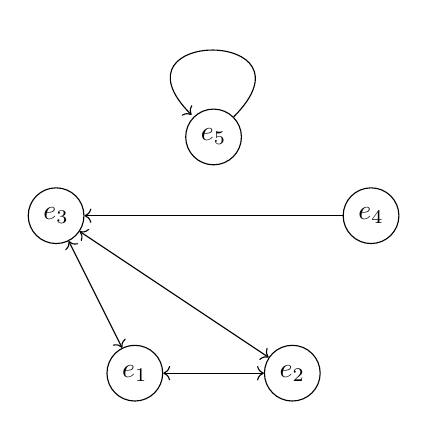
\begin{tikzpicture}
    \node[shape=circle,draw=black] (A) at (1,0) {$e_1$};
    \node[shape=circle,draw=black] (B) at (3,0) {$e_2$};
    \node[shape=circle,draw=black] (C) at (0,2) {$e_3$};
    \node[shape=circle,draw=black] (D) at (4,2) {$e_4$};
    \node[shape=circle,draw=black] (E) at (2,3) {$e_5$};
         \path [<->] (E) edge [loop] node {} (B);
     \path [<->] (A) edge node {} (B);
     \path [<->] (A) edge node {} (C);
     \path [<->] (B) edge node {} (C);
     \path [->](D) edge node {} (C);
\end{tikzpicture}
\]
The evolution algebra associated with G is
\begin{gather*}
e_1^2 = e_2+ e_3 \qquad e_2^2 =e_1+e_2 \qquad e_3^2 = 0\\
e_4^2 = e_3 \qquad e_5^2= e_5
\end{gather*}
Conversely, if we have a graphicable evolution algebra like
\begin{gather*}
e_1^2 = e_2 + e_4 \qquad e_2^2 =e_4 \qquad e_3^2 = e_2+e_4 \qquad e_4^2 = 0
\end{gather*}
The graph associated to this evolution algebra is
\[
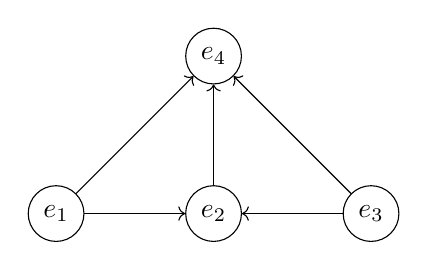
\begin{tikzpicture}
    \node[shape=circle,draw=black] (A) at (0,0) {$e_1$};
    \node[shape=circle,draw=black] (B) at (2,0) {$e_2$};
    \node[shape=circle,draw=black] (C) at (4,0) {$e_3$};
    \node[shape=circle,draw=black] (D) at (2,2) {$e_4$};
     \path [->] (A) edge node {} (D);
     \path [->] (B) edge node {} (D);
     \path [->] (C) edge node {} (D);
	\path [->] (A) edge node {} (B);
     \path [->] (C) edge node {} (B);
\end{tikzpicture}
\]
\end{ejem}



\section{Endowing evolution algebras with properties of graphs. First definitions and results}

In this section we provide the evolution algebras with discrete
 properties

\vspace{0.1cm}

From here on, $E$ denotes an evolution algebra with respect to a
set of generators \,\,$\Delta = \{e_i \mid i \in \Lambda \}$,
where $\Lambda$ is a finite set of indices. $G$ will denote the
graph associated with $E.$


\begin{defi}
The {\em skeleton} of $E$, which we will denoted by $B(E),$ is
the evolution algebra whose structure constants are

\begin{equation*}
b_{ij}= \left\{
\begin{array}{lc}
1, & \text{if } a_{ij}\neq 0,\\
0, & \text{if } a_{ij}= 0.
\end{array}
\right.
\end{equation*}
\end{defi}

\begin{ejem} Let consider the evolution algebra E defined by the brackets
\begin{align*}
e_1^2= & 4e_2-8e_3 &  e_2^2= & 15e_1+16e_3 \\
e_3^2 = &  23e_1-42e_3   &  e_4^2= &-815e_3
\end{align*}
The skelenton of E is defined by the brackets
\begin{align*}
e_1^2= & e_2+e_3 &  e_2^2= & e_1+e_3 \\
e_3^2 = &  e_1+e_3 &    e_4^2= &e_3
\end{align*}
and we can asociate the graph
\[
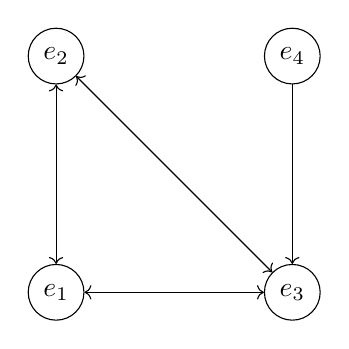
\begin{tikzpicture}
    \node[shape=circle,draw=black] (A) at (0,0) {$e_1$};
    \node[shape=circle,draw=black] (B) at (0,3) {$e_2$};
    \node[shape=circle,draw=black] (C) at (3,0) {$e_3$};
    \node[shape=circle,draw=black] (D) at (3,3) {$e_4$};
    
     \path [<->] (A) edge node {} (B);
     \path [<->] (A) edge node {} (C);
     \path [<->] (B) edge node {} (C);
     \path [->](D) edge node {} (C);
\end{tikzpicture}
\]
\end{ejem}

The following result follows immediately from the previous
definition

\begin{prop}
The skeleton of an evolution algebra is a graphicable
evolution algebra.
\end{prop}

\begin{nota}
Unless otherwise stated, when we deal with the graph $G$
associated with $E$, we mean the graph associated with $B(E).$ In
this way and although this manner is not bijective, a graph can be
associated with any evolution algebra.
\end{nota}




\begin{defi}
Let $W$ be a vector subspace of $E$ generated by $\{e_i \mid i \in
A\}$. The {\em evolution subgraphic algebra} of $W$ is the one
that its structure constants are

\begin{equation*}
b_{ij}= \left\{
\begin{array}{lc}
a_{ij}, & \text{if } j \in A\\
0, & otherwise.
\end{array}
\right.
\end{equation*}
\end{defi}

\begin{ejem}
Let $E$ be an evolution graphicable and $G$ be its associated
graph. The evolution subgraphic algebras of $E$ are the algebras
which are associated, in the natural way, with the subgraphs of
$G.$
\end{ejem}

Note that according to this definition, the following result is
immediate. However, the converse in not true, in general.

\begin{prop}
If $E_1$ is a evolution subalgebra of E, then $E_1$ is a
subgraphic algebra of $E.$
\end{prop}

As we have just indicated, the converse of this result in not
true, in general. Let us see it with the following counterexample

\begin{ejem}
Let consider the evolution algebra defined by the
brackets
\begin{align*}
e_1^2=e_2+e_3 &  & e_2^2= & e_1+e_3 \\
e_3^2 = e_1+e_3 &  &  e_4^2= &e_3
\end{align*}

It is obvious that the set generated by $\{e_1,e_3\}$ is not a
evolution subalgebra of $E.$ The evolution subgraphic algebra
 with this set is
\begin{align*}
e_1^2= e_3 &  & e_3^2 = e_1+e_3
\end{align*}
\end{ejem}


\begin{thm}
There exists a bijective correspondence between the evolution
subgraphic algebras of $E$ and the subgraphs of $G.$
\end{thm}

And an immediate consequence of the previous result is the
following

\begin{cor}
There exists a injective correspondence between the evolution
subalgebras of $E$ and the subgraphs of $G.$
\end{cor}

\section{The concept of adjacency in evolution algebras}

\begin{defi}
Let $e_i$ and $e_j$ two generators of an evolution algebra $E.$
The generator $e_i$ is said to be {\em adjacent} to the generator
$e_j$ if the corresponding structure constant $a_{ij}$ is
different from $0.$
\end{defi}

\begin{ejem} Let consider the evolution algebra E defined by the brackets
\begin{align*}
e_1^2= & 2e_2-3e_3 &   e_2^2= & 5e_1+7e_3 \\
e_3^2 = &  11e_1-13e_3 &   e_4^2= &-17e_3
\end{align*}
For instance, we can say $e_1$ is adjacent to $e_2$ or $e_4$ is adjacent to $e_3$, althought $e_3$ is not adjacent to $e_4$.
\end{ejem}
The following results are deduced directly from this definition


\begin{prop}
Let $E$ be an evolution algebra and $G$ its associated graph. These 
two statements are equivalent
\begin{itemize}
\item The generator $e_i$ of $E$ is adjacent to the generator $e_j.$
\item The vertex $e_i$ of $G$ is adjacent to the vertex $e_j.$
\end{itemize}
\end{prop}



\begin{defi}
The evolution algebra $E$ is called {\em simple graphically} if
the condition $e_i$ is adjacent to $e_j$ implies that $e_j$ is
adjacent to $e_i$. Tian called this concept \textit{occurs}. 
\end{defi}

\begin{ejem} An example of this kind of algebra is
\begin{align*}
e_1^2= & e_2+e_3 &   e_2^2= & e_1+e_3  &   e_3^2= & e_1+e_2 
\end{align*}
An its associated graph is
\[
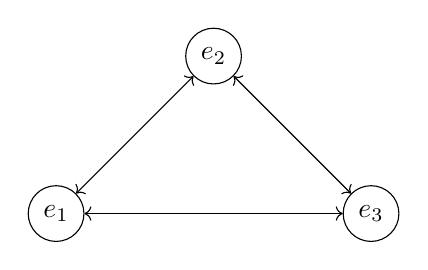
\begin{tikzpicture}

    \node[shape=circle,draw=black] (A) at (0,0) {$e_1$};
    \node[shape=circle,draw=black] (B) at (2,2) {$e_2$};
    \node[shape=circle,draw=black] (C) at (4,0) {$e_3$};
    
     \path [<->] (A) edge node {} (B);
     \path [<->] (A) edge node {} (C);
     \path [<->] (B) edge node {} (C);
\end{tikzpicture}
\]
\end{ejem}
\begin{prop} \label{Prop4}
Let $E$ be an evolution algebra and
let $e_i$, $e_j$ be two generators of $E$ such that $e_j^2 \neq
0.$ Then, $e_i$ is adjacent to $e_j$ if and only if
\begin{gather*}
e_i^2 e_j \neq 0.
\end{gather*}
\end{prop}

\begin{ejem} The evolution algebra E defined by the brackets
\begin{align*}
e_1^2 = e_2 &  &  e_2^2 = & e_3 &  & e_3^2=  e_4  \\
e_4^2 = e_5 &  &  e_5^2 = & e_6 &  & e_6^2= e_1+e_2+e_4 
\end{align*}
is an example of this kind of algebra. However, the evolution algebra E defined by the brackets
\begin{align*}
e_1^2= & e_2+e_3   & e_2^2= & e_1+e_3 \\
e_3^2 = &  e_1 &   e_4^2= &  0
\end{align*}
isn't it.
\end{ejem}

\begin{prop}
Let $E$ be an evolution algebra and $G$ its associated graph.
Then, $E$ is simple graphically if and only if $G$ is a simple
graph.
\end{prop}

\begin{ejem}
Let consider the evolution algebra defined by the brackets
\begin{align*}
e_1^2=e_2+e_3 & &e_2^2=e_1+e_3 & & e_3^2 = e_1.
\end{align*}

It is immediate to see that $e_1$ is adjacent to $e_2$  and that
$e_1^2 e_2 = e_2^2 = e_1 + e_3$. However, $e_3$ is not adjacent to
$e_2$, because $a_{23}=0,$ or,  equivalently, $e_3^2 e_2 = 0$.
\end{ejem}


\begin{defi} Let $E$ be an evolution algebra. The outdegree of $e_i$ (denoted by $\delta(e_i)$) is the number of generators
adjacent to the generator $e_i.$ 
\end{defi} 
\begin{prop}
Let $E$ be a finitely generated evolution algebra with
$|\Lambda|=n.$ Then,
\begin{gather*}
\sum_{i\in\Lambda}\delta(e_i) \leq n(n+1)
\end{gather*}
\end{prop}


\section{Walks in evolution algebras}

\begin{defi}
Let $C = \{e_{i_1},\dotsc,e_{i_k}\}$ an ordered sequence of
generators of an evolution algebra $E.$ The {\em walk operator}
$d$ of $E$ is defined as
\begin{equation*}
\gamma(\{e_{i_1},\dotsc,e_{i_k}\})= (((e_{i_1}^2
e_{i_2})e_{i_3})\cdots e_{i_k}) = e_{i_1} \prod_{j=1}^k e_{i_j}
\end{equation*}
\end{defi}

Let us see an example of this novel concept

\begin{ejem}
Let us consider the evolution algebra defined by
\begin{align*}
e_1^2=e_2+e_3 &  & e_2^2= & e_1+e_3 \\
e_3^2 = e_1+e_3 &  &  e_4^2= &e_3
\end{align*}
\noindent and let consider the subsets of generators $C_1 =
\{e_{4},e_{3},e_1\}$ and $C_2 =\{e_{2},e_{3},e_4\}.$ Then
\begin{gather*}
\gamma(C_1) = (e_4^2 e_3)e_1 = e_3^2 e_1 = (e_3 + e_1)e_1 = e_2+e_3\\
\gamma(C_2) = (e_2^2 e_3)e_4 = ((e_1+e_3)e_3)e_4 = e_3^2 e_4 = 0
\end{gather*}
\end{ejem}

\begin{prop}
Let $C = \{e_{i_1},\dotsc,e_{i_k}\}$ an ordered sequence of
generators of an evolution algebra $E.$ They are equivalent
\begin{itemize}
\item $\gamma(e_{i_1},\dotsc,e_{i_k})\neq 0$.
\item $\forall j=1,\dotsc,k-1$, $e_{{i_j}}$ is adjacent to $e_{i_{j+1}}$ and $e_{i_k}^2\neq 0$.
\end{itemize}
\end{prop}

\begin{defi}
An evolution algebra $E$ is said to be {\em non-negative} when all
its structure constants are non-negative.
\end{defi}


\begin{defi}
Let $E$ be an evolution algebra with respect o a set of generators
$\{e_i \mid i \in \Lambda \}$ and let
$C=\{e_{i_1},\dotsc,e_{i_k}\}$ be  an ordered sequence of
generators of $E.$
\begin{itemize}
\item $C$ is said to be a {\em walk} in $E$ if $e_i$ is adjacent to $e_{i+1},$
for all $i \in \Lambda$.

\item $C$ is said to be a {\em trail} in $E$ if $C$ is a walk
verifying that if two generators are consecutive in $C$, then both
are consecutive only one time in $C.$

\item $C$ is said to be a {\em circuit} in $E$ if $C$ is a trail
such that $e_{i_1}=e_{i_k},$ for all $i,k \in \Lambda.$

\item $C$ is said to be a {\em path} in $E$ if $C$ is a circuit
such that $e_{i_j} \neq e_{i_k},$ for all $j,k \in \Lambda.$

\item A path in which the first and the last generator coincide is called {\em cycle}.
\end{itemize}
\end{defi}

\begin{nota}
Note that in a walk you can move around from generator to generator by
sing the adjacency. In the case of a trail, you cannot
move around for an adjacency already used.
\end{nota}

We are now going to illustrate some parts of the previous
definition with the following

\begin{ejem}
Let consider the volution algebra $E$ defined by
\begin{align*}
e_1^2 & =e_2+e_5          &  e_2^2 & = e_1+e_3  \\
e_3^2 & = e_4+e_6           &  e_4^2 & = e_1+e_2+e_3 \\
e_5^2 & = e_2+e_3+e_6   &  e_6^2 & = e_3+e_5+e_4
\end{align*}

The subsets
\begin{equation*}
C_1 = \{e_1,e_2,e_3\} \quad C_2 = \{e_3,e_6,e_5,e_2\}
\end{equation*}
\noindent are trails.

\vspace{0.1cm}

The subsets
\begin{equation*}
C_3 = \{e_1,e_2,e_1,e_5\} \quad C_4 =
\{e_2,e_3,e_4,e_1,e_5,e_6,e_4,e_3\}
\end{equation*}
\noindent are not trails.
\end{ejem}

\begin{prop}
Let $E$ be an evolution algebra. Then, the sequence of vertices
$\{e_1,\dotsc,e_n\}$ is a walk in $E$ (respectively trail,
circuit, path or cycle) if and only if the sequence of vertices
$\{e_1,\dotsc,e_n\}$ is a walk in $G$ (respectively, trail,
circuit, path or cycle).
\end{prop}

\noindent {\em Proof}

The proof is an immediate consequence of Proposition \ref{Prop4}.
\hfill $\Box$

\vspace{0.1cm}

It is convenient to say that some of these concepts constitute a
generalization of others already introduced by Tian. For instance,
he defined the {\em algebra of walk} of dimension $p$ as the
evolution algebra defined, with respect to the set of generators
$\{e_1,e_2,\dotsc,e_p\}$ by
\begin{equation*}
\begin{array}{lll}
e_1^2    & =    &     e_2,  \\
e_2^2    & =    &    e_1 + e_3, \\
         &\vdots     &      \\
e_{p-1}^2  &  =     &      e_{p-2} + e_p, \\
e_p^2      &  =     &     e_{p-1} \\
\end{array}
\end{equation*}


\vspace{0.1cm}

Let observe that once such a definition is given, it is trivial to
see that $C=\{e_1,e_2,\dotsc,e_p\}$ is a walk (in fact, it is also
a trail and a path) such that we have defined them.

\vspace{0.1cm}

Tian also defined the {\em cyclic algebra} of dimension $p$ as the
evolution algebra having $\{e_1,e_2,\dotsc,e_p\}$ as the set of
generators and it is defined by
\begin{equation*}
\begin{array}{lll}
e_1^2    & =    &    e_p + e_2,  \\
e_2^2    & =    &    e_1 + e_3, \\
         &\vdots     &      \\
e_{p-1}^2  &  =     &      e_{p-2} + e_p, \\
e_p^2      &  =     &     e_{p-1} + e_1. \\
\end{array}
\end{equation*}

\vspace{0.1cm}

Let note that it is very easy to see that
$C=\{e_1,e_2,\dotsc,e_p,e_1\}$ is a cycle.


\section{Operator L}

We present in this section an operator and new properties and concepts using the operator L, already introduced by 
Tian in \cite{book}. From here on, we will suppose that evolution algebras are defined over $\mathbb{R}.$ We recall the definition of L.

\begin{defi}
Let $\{e_1, \ldots, e_n\}$ be a set of generators of an evolution algebra $E.$ Let consider the element 
$x = \sum_{k\in\Lambda} x_k e_k,$ of $E.$ We define the operator 
\begin{gather*}
L: E \rightarrow E\\
L(x) = \sum_{k\in\Lambda} x_k e_k^2 = \sum_{k\in\Lambda} \left(\sum_{j\in\Lambda} x_j a_{jk}\right)e_k  
\end{gather*}
\end{defi}

It is easy to see that $L$ is a linear operator.


\begin{defi}
Let $e_i,e_j$ two generators of $E.$ If $\delta(e_j)\neq 0$, we define the {\em walk operator} of length $n$ from 
$e_i$ to $e_j,$ $\Gamma^n(e_i,e_j),$ as
\begin{gather*}
\Gamma^n(e_i,e_j) = \gabs{\frac{L^n(e_i)\cdot e_j}{\delta(e_j)}}
\end{gather*}
where $|x| = \sum_{k\in\Lambda}|x_k|$.
\end{defi}

\begin{nota}
If $e_i=e_j,$ the previous defined operator will be denoted by $\Gamma^n(e_i).$
Moreover, if different algebras are considered, $\Gamma^n_E(e_i,e_j)$ will denote 
the walk operator of length $n$ from $e_i$ to $e_j$ with the inner law on $E.$
\end{nota}

\begin{lemma}
Let E be a graphicable evolution algebra where every generator verifies $\delta(e_i)\neq 0$. Then $\sum_{j\in\Lambda}a_{ij} = \delta(e_i)$ and
\[ \Gamma^{n+1}(e_i,e_j) = \sum_{k\in\Lambda} a_{ik} \Gamma^n(e_k,e_j)\]
\end{lemma}
\noindent {\em Proof}

The first statement is trivial. Then we consider
\begin{gather*}
\Gamma^{n+1}(e_i,e_j) = \gabs{\frac{L^{n+1}(e_i)\cdot e_j}{\delta(e_j)}} = \sum_{k\in\Lambda}a_{ik}\gabs{\frac{L^n(e_k)\cdot e_j}{\delta(e_j)}} = \sum_{k\in\Lambda} a_{ik}\Gamma^n(e_k,e_j)
\end{gather*}
\hfill $\Box$
\begin{prop}
Let $E$ be a graphicable evolution algebra where every generator verifies $\delta(e_i)\neq 0$, then 
\begin{gather*}
L^n(e_i) = \sum_{j\in\Lambda} \Gamma^n(e_i,e_j) e_j.
\end{gather*}
\end{prop}
\noindent {\em Proof}

We will proceed by induction.

If $n=1,$ then 

\begin{gather*}
\Gamma(e_i,e_j) = \gabs{\frac{L(e_i) e_j}{\delta(e_j)}}=  \frac{1}{\delta(e_j)}\gabs{{\sum_{j\in \Lambda} \left(a_{ij}e_j\right) e_j}} = \\ = \frac{a_{ij}}{\delta(e_j)} \gabs{\sum_{k\in \Lambda} a_{jk}e_k}=  \frac{a_{ij}\sum_{k\in\Lambda}a_{jk}}{\delta(e_j)}=a_{ij}
\end{gather*}
Let us suppose that the result is true for $n=k$

Then, for $n=k+1$ we have
\begin{gather*}
L^{k+1}(e_i) = L^k((L(e_i)) = \sum_{j\in\Lambda}a_{ij}L^k(e_j) =  \sum_{j\in\Lambda}a_{ij}\sum_{k\in\Lambda} \Gamma^k(e_j,e_k) e_k = \\ = \sum_{j\in\Lambda} \left(\sum_{k\in\Lambda} a_{ik} \Gamma^k(e_k,e_j)\right)e_j  = \sum_{j\in\Lambda} \Gamma^k(e_i,e_j) e_j 
\end{gather*}
\hfill $\Box$

\begin{lemma}
Let $E$ be a  finitely generated non-negative evolution algebra and $E'$ a subgraphic evolution generated by $\{e_i \mid i \in A\}.$ Then, for all 
$m \in \mathbb{N}$ and for all generators $e_i,e_j$ of $E'$ where $\Gamma^n$ is defined, it is verified that
\begin{gather*}
\Gamma^n_{E'}(e_i,e_j) \leq \Gamma^n_{E}(e_i,e_j)
\end{gather*}
\end{lemma}


\noindent {\em Proof}

We will proceed by induction.

If $n=1,$ then 
\begin{gather*}
L(e_i)_{E} = \sum_{j \in \Lambda} a_j e_j^2 = \sum_{j \in
\Lambda} b_j e_j  \qquad L(e_i)_{E'} = \sum_{k \in A} c_k e_k^2 =
L(e_i)_{E'} = \sum_{k \in A} d_k e_k
\end{gather*}
\noindent due to that $E$ is non-negative and that 
$a_i\geq c_i\geq 0$ and $b_i \geq d_i \geq 0,$ for all $i \in A,$ by the definition of 
subgraphic algebra.

Let us suppose that the result is true for $n=k.$

Then, for $n=k+1$ we have
\begin{gather*}
{\delta(e_j)} \Gamma^{k+1}_{E'}(e_i,e_j) = \gabs{L^{k+1}_{E'}(e_i)\cdot e_j} = \gabs{L^{k}_{E'}(L_{E'}(e_i))\cdot e_j} =\\ \gabs{L^k_{E'}\left(\sum_{s\in A} a_{is} e_s\right)\cdot e_j} 
= \sum_{s\in A} a_{is} \gabs{ L^k_{E'}(e_s)\cdot e_j} = \delta(e_j) \sum_{s\in A} a_{is} \Gamma^k_{E'}(e_s,e_j) \leq  \\ 
\leq \delta(e_j)  \sum_{s\in A} a_{is} \Gamma^k_{E}(e_s,e_j)  \leq \delta(e_j)  \sum_{s\in \Lambda} a_{is} \Gamma^k_{E}(e_s,e_j) = {\delta(e_j)}  \Gamma^{k+1}_{E}(e_i,e_j)
\end{gather*}
\hfill $\Box$


\section{Walks}

In this section, when we mention the graph $G$ associated with the
evolution algebra $E$ we are reffering to the graph naturally associated 
to $E$ in the natural way and not the graph associated with $B(E),$ as 
we have done in previous sections. 



\begin{prop}
Let $E$ be a  graphicable evolution algebra and let
$e_i$ one of its generators. If
\begin{gather*}
\Gamma^n(e_i)=\sum_{k\in\Lambda} \nu_{ij}e_k
\end{gather*}
\noindent is obtained when applying $n$ times $\Gamma^n$ on $e_i,$
then the coefficients $\nu_{ij}$ represent the number of walks
different of length $n$ which there are from $e_i$ to $e_k.$
\end{prop}

\noindent {\em Proof}

We proceed by induction. For $n=1,$ the result is directly
obtained by using the natural association between graphs and
evolution algebras.

Let us suppose that the result is true for $n=k.$ Let consider the
set  $\Delta=\{e_j \mid e_j \, \, \text{is \, adjacent \,to} \,\,
e_k\}.$ The induction hypothesis assures that $\Gamma^k(e_i,e_j)$
gives the walks of length $n$ from $e_i$ to $e_j$. Then, it
suffices to consider that all the walks of length $n$ from
$e_i$ to $_k$ are the sum of the walks going from $e_i$ to $e_j$
multiplied by those going from $e_j$ to $e_k$. \hfill $\Box$


\begin{cor}
Let $E$ be a  graphicable evolution algebra and let
$e_i, e_j$ be two generators of $E$ and let consider
$A^n=\left(a_{ij}^n\right),$ where $A$ is the adjacency matrix of
the graph associated with $E.$ Then, the following expression is
hold
\begin{gather*}
L^n(e_i)=\sum_{j\in \Lambda} a_{ij}^n e_j
\end{gather*}
\end{cor}

\noindent {\em Proof}

It is an immediate consequence of the previous proposition and of
the properties on $A.$ \hfill $\Box$

\begin{cor}
The number of walks of length $n$ existing between two
vertices of a complete graph $K_m$ is

$$
\left \{
\begin{array}{ll} \dfrac{(m-1)^n+(-1)^n(m-1)}{m}, &  \quad  \mbox{{\rm if
the initial and final vertices
coincide}}, \\
& \\
 \dfrac{(m-1)^n+(-1)^n(m-1)}{m}+(-1)^{n+1}, &  \quad \mbox{{\rm if the initial and
final vertices are different}}. \\
\end{array}
\right.
$$
\end{cor}



\section{Cycles}

\begin{prop} Let $E$ be a graphicable evolution algebra. The
number of cycles of length $3$ containing the generator $e_i$ is
$\dfrac{\Gamma^3(e_i)}{2}$.
\end{prop}

\begin{prop} Let $E$ be the evolution algebra associated with the cycle $C_m$ of length $m.$ Then,

$$
\left \{
\begin{array}{ll}
\Gamma^n(e_i) = 2, &  \quad \mbox{{\rm if G is a cycle of length odd}}, \\
 & \\
\Gamma^n(e_i) = 2 + \binom{n}{n/2}, & \quad \mbox{{\rm if G is a
cycle
of length even}}. \\
\end{array}
\right.
$$
\end{prop}

Let us note that these two values are two times the number of
partitions of the set of vertices which can be induced by
endomorphims on cyclic graphs of length odd and even,
respectively (this result can be found in \cite{numeroraro}).


\section{Hamiltonian evolution algebras}

\begin{defi}
An evolution algebra $E$ is called {\em Hamiltonian} if there
exist a cycle which contains all the generators.
\end{defi}

\begin{ejem} An example of an hamiltonian evolution algebra E is defined by the brackets
\begin{align*}
e_1^2= & e_2+e_3 &  e_2^2= & e_2+e_3 \\
e_3^2 = &  e_1+e_4   &  e_4^2= & e_1
\end{align*}
and we can asociate the next graph with a hamiltonian cycle in red
\[
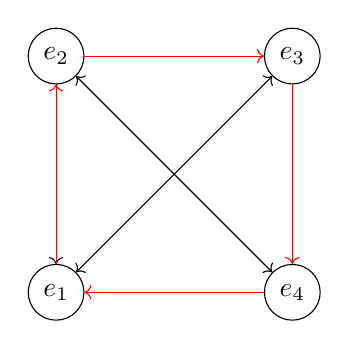
\begin{tikzpicture}
    \node[shape=circle,draw=black] (A) at (0,0) {$e_1$};
    \node[shape=circle,draw=black] (B) at (0,3) {$e_2$};
    \node[shape=circle,draw=black] (C) at (3,0) {$e_4$};
    \node[shape=circle,draw=black] (D) at (3,3) {$e_3$};
    \path [->] (B) edge node {} (A);
    \path [<->] (A) edge node {} (D);
    \path [<->] (B) edge node {} (C);
\begin{scope}[
              every edge/.style={draw=red}]
    \path [->] (A) edge node {} (B);
    \path [->] (B) edge node {} (D);
    \path [->] (C) edge node {} (A);
    \path [->] (D) edge node {} (C);
\end{scope}

\end{tikzpicture}
\]
\end{ejem}
The following result is an immediate consequence of the previous
definition

\begin{prop}
An evolution algebra is Hamiltonian if and only if its associated
graph is Hamiltonian.
\end{prop}

\begin{prop}
A n-dimensional evolution algebra $E$ is Hamiltonian if and only
if there exist $\sigma \in S_n$ such that the set
$C=\{e_{\sigma(1)},\dotsc,e_{\sigma(n)}\}$ verifies that
\begin{gather*}
\gamma(C)\cdot e_{\sigma(1)} = \left(e_{\sigma(1)} \prod_{i=1}^{n}
e_{\sigma(i)}\right)  e_{\sigma(1)} \neq 0.
\end{gather*}
\end{prop}

\begin{prop}
Let E be a Hamiltonian n-dimensional evolution algebra. Then every
generator verifies
\[
\Gamma^n(e_i) \geq 
\begin{cases}
2 & \text{if n is odd}\\
2+\binom{n}{n/2} &\text{ if n is even}
\end{cases}
\]
\end{prop}
It's an obvious consequence of Lemma 5.6 and Proposition 7.2.
\begin{prop}
Let E be a Hamiltonian n-dimensional evolution algebra. Then every
generator verifies
\[
\Gamma^n(e_i) \geq \underset{d<n}{\sum_{d\mid n}}2^{\frac{n}{d}-1}\Gamma^d(e_i) + 2
\]
\end{prop}
%// piensa esto ma�ana: tiene que existir un ciclo de longitud n,
%es decir, el coeficiente de Gamma^n(e_i) tiene que ser mayor que 1. Es m�s,
%intenta eliminar los casos triviales para una mejor acotaci�n, algo rollo
%mayor que delta(e_i) o as�.

\section{Distances, circumference, diameter, radio, girth,
eccentricity, center and geodesics in graphicable evolution
algebras}

In this section we firstly define the concept of distance between
two generators of an evolution algebra and we use it to introduce
the diameter, the radio, the girth, the circumference and
the center of the algebra and the eccentricity de its
generators.

\begin{defi} Let $E$ be a graphicable evolution algebra. The {\em distance} between two generators $e_i$ and $e_j,$ denoted by $d(e_i,e_j)$ is defined as
the length of the minor walk which links them.
\end{defi}

Note that this concept in evolution algebras is the same as the
corresponding in the associated graph.

\begin{defi} Let $E$ be a graphicable evolution algebra. Let us consider the set $C$ of cycles of $E$ and the set $L$ of the lengths
of these cycles (if there exist, logically). The minimum and the
maximum  element of $L$ are called, respectively, the {\em
girth} and the {\em circumference} of $E.$
\end{defi}


\begin{defi} Let $e_i$ be a generator of a graphicable evolution algebra $E$. The {\em eccentricity} of $e_i$ is the greater distance between $e_i$ and another
generator of $E.$
\end{defi}

\begin{defi} The generators of a graphicable evolution algebra with minor eccentricity are called {\em central generators}. The set of the
central generators of $E$ is called the {\em center} of the
algebra.
\end{defi}

\begin{defi} The minor (greater, resp.) of the eccentricities of the generators of a graphicable evolution algebra $E$ is called {\em radio
(diameter), resp.} of the algebra.
\end{defi}

\begin{defi} The {\em geodesics} of a graphicable evolution algebra $E$ are those
walks in the algebra whose length coincides with the
distance between the initial and final generators of such walks.
\end{defi}


\begin{nota}
According to these definitions, it is clear that the diameter
$d$ of the algebra is the length of the greater of its
geodesics and that, if $r$ denotes the radio, then $ r \leq d \leq
2\, r.$
\end{nota}


\begin{prop}
Let $E$ be an evolution algebra, defined with
respect to a generator set $\{e_i \mid i \in \Lambda \},$
associated with a graph $G.$ Then, the distance between two
generators of $E$ is

\begin{gather*}
d(e_i,e_j)=\min \{n\mid L^n(e_i,e_j)\neq 0\}
\end{gather*}
\noindent considering $L^0$ as the identity.
\end{prop}


\section{Algebraic connection}
\subsection{Strong and weak connection}
\begin{defi}
An evolution algebra is said to be {\em strongly connected} or
simply {\em connected} if each pair of generators $e_i$ and $e_j$
is joined by a walk. If the evolution algebra is not connected, it
is called {\em disconnected}.
\end{defi}

\begin{defi}
An evolution algebra (resp. graph) is called {\em weakly
connected} if when converting the algebra (resp. graph) in
graphically simple (resp, simple), it becomes connected.
\end{defi}

\begin{ejem} An example of a weakly connected graph that isn't strongly connected
\begin{align*}
e_1^2= & e_2+e_4 &  e_2^2= & 0 \\
e_3^2 = &  e_2  &  e_4^2= & e_2
\end{align*}
\[
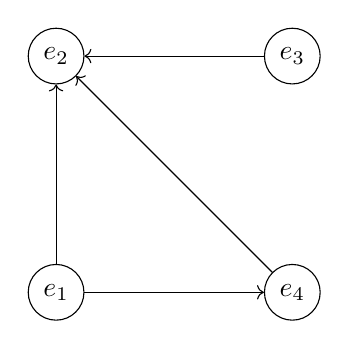
\begin{tikzpicture}
    \node[shape=circle,draw=black] (A) at (0,0) {$e_1$};
    \node[shape=circle,draw=black] (B) at (0,3) {$e_2$};
    \node[shape=circle,draw=black] (C) at (3,0) {$e_4$};
    \node[shape=circle,draw=black] (D) at (3,3) {$e_3$};
    \path [->] (A) edge node {} (B);
    \path [->] (C) edge node {} (B);
    \path [->] (D) edge node {} (B);
    \path [->] (A) edge node {} (C);
\end{tikzpicture}
\]
\end{ejem}


\begin{nota}
The intuitive notion of weak connection involves that each
generator $e_i$ of the algebra (resp, vertex in the graph) is,
 either adjacent to another generator (resp, vertex) $e_j$ or there exists another generator $e_k,$ which is adjacent to
$e_i,$ that is, for each pair of generators $e_i$ and $e_j$ there
exists a walk between them.
\end{nota}

\begin{prop}
Let $E$ be an evolution algebra. $E$ is connected (resp. weakly
connected) if and only if the graph associated with the subalgebra
$B(E)$ is connected (resp. weakly connected).
\end{prop}

\noindent {\em Proof}


Ii is immediate by using Proposition 4 and the fact that $E$ and
$B(E)$ share adjacencies. \hfill $\Box$.

\begin{cor}
Let $E$ be an $n$-dimensional graphically simple evolution
algebra. If
\begin{gather*} \sum_{i\in\Lambda} \delta(e_i) < 2n-2
\end{gather*}
\noindent is verified, then $E$ is disconnected.
\end{cor}

\noindent {\em Proof}

According to the previous result, only it is needed to check the
connectivity in the associated graph. Since that the graph has
less than $2n - 2$ adjacencies by hypothesis, it has less than
$n-1$ edges. \hfill $\Box$.

\begin{defi}
Let $E_1$ be an evolution subalgebra of an evolution algebra
$E.$ $E_1$ is said to be a {\em strongly (weakly) connected component}
of $E$ if $E_1$ is strongly (weakly) connected there is not another
evolution subalgebra $E_1 \subset E_2 \subset E$ such that $E_2$
is (weakly) connected.
\end{defi}


\subsection{Simplicity}

Let us recall that every evolution subalgebra of an evolution
algebra is an ideal of the algebra and conversely. Besides, in
this subsection we will take into consideration the following
concepts of simple and semisimple evolution algebra, already seen
in \cite{book}.

\begin{defi} Let $E$ be an evolution algebra and $E_1$ an evolution subalgebra of $E.$ $E_1$ is said to be {\em proper} if it is neither $\{0\}$ nor E.
\end{defi}
\begin{defi}

An evolution algebra $E$ is {\em simple} if it has no proper
evolution subalgebras.
\end{defi}

\begin{defi}
An evolution algebra is {\em connected} if it cannot be expressed
as a sum of proper evolution subalgebras.
\end{defi}

\begin{defi}
An evolution algebra $E$ is {\em semisimple} if it can be
decomposed as a direct sum of simple evolution subalgebras.
\end{defi}

The following result is an immediate consequence of these
definitions.

\begin{ejem} The evolution algebra of Example 10.3 isn't simple ($\{e_2\}$ generate a proper subalgebra), is connected and isn't semisimple.
\begin{align*}
e_1^2= & e_2+e_4 &  e_2^2= & 0 \\
e_3^2 = &  e_2  &  e_4^2= & e_2
\end{align*}
\end{ejem}
\begin{prop} Let $E$ be an evolution algebra. $E$ is simple,
semisimple or connected if and only if $B(E)$ is simple,
semisimple or connected, respectively.
\end{prop}




\begin{prop}[Characterization of connected algebras] Let $E$ be an evolution algebra. $E$ is connected if and only if it is weakly connected.
\end{prop}

\noindent {\em Proof}

Note that $E$ is non-connected if and only if it is a direct sum of two evolution subalgebras, which, by definition, are generated by two sets of different generators 
$\Delta_1$ and $\Delta_2$ different. \hfill $\Box$

\begin{prop}Let $E$ an evolution algebra E. $E$ is simple if and only if E is strongly connected.
\end{prop}

\noindent {\em Proof}

Let us suppose that $E$ is strongly connected. By reductio ad absurdum, if $E$ is not simple, then there would exist an evolution subalgebra 
$E_1 \subset E$ with a set of generators $\Delta_1.$ Then, for all $e_i \in \Delta\setminus \Delta_1$ and for all $e_j \in
\Delta_1,$ it cannot exist a walk joining $e_j$ and $e_i,$ since that if this walk exists, $E_1$ cannot be a subalgebra of $E,$ for not being closed for the 
product). It is in contradiction with the hypothesis of being $E$ strongly connected.

Conversely, let us suppose that $E$ is simple. If E is simple then it is connected and weakly connected. If it is non-strongly connected, there will exist $e_i,e_j \in \Delta$ such that there is no walk from $e_i$ to $e_j$. Then exists a proper subalgebra which contains $e_j$ and doesn't contain $e_i$.
\hfill $\Box$

\begin{prop} [Characterization of simple algebras]
If E is graphically simply then be connected, simple, weakly connected and strongly connected are equivalent.
\end{prop}
\noindent {\em Proof}

If E is graphically simply then E is weakly connected if and only if E is strongly connected. By the Proposition 10.14, it is equivalent to be connected. We know strongly connected implies simple. If E is simple then is connected.
\hfill $\Box$


\begin{cor} [Characterization of semisimple algebras]
Let E an evolution algebra. E is semisimple if and only if it's associated graph is an union of strongly connected graphs.
\end{cor}


\begin{thm} Let $E$ be a finitely generated semisimple evolution algebra. If $w(E)$ denotes de number of weakly connected components of $E$, the the number of evolution subalgebras of $E$ is  $2^{w(E)}$.
\end{thm}


\noindent {\em Proof}

Indeed, there are $w(E)$ simple evolution subalgebras of $E.$ Any other subalgebra of $E$ must be a direct sum of them, apart from 
$\{0\}$ and the own $E.$ It is easy to see that 
\begin{gather*}
\sum_{k=0}^{w(E)} \binom{w(E)}{k} = 2^{w(E)}  
\end{gather*}
\hfill $\Box$

\begin{ejem}
The graphically simple graphicable algebras, that is, those graphicable algebras whose associated graph is simple, constitute a example of algebras verifying the previous result.
\end{ejem}



\newpage






\begin{thebibliography}{99}


\bibitem{bollo} Bollob�s, B., Graphs Theory, Springer Verlag, New York, 1979.

\bibitem{cabrera} Cabrera Y., Siles, M. and Velasco, M. V.,  Evolution algebras of arbitrary dimension and their decompositions, {\em Linear Algebra and its Applications}, {\bf 495}  (2016), 122�162.



\bibitem{elduque} Elduque, A. and Labra, A.,  Evolution algebras and graphs, {\em Journal of Algebra and Its Applications}
{\bf 14}: 7 (2015), 1550103  (10 pages).


\bibitem{harary} Harary, F., Graph Theory, Addison Wesley, Reading, Mass., 1969.

%\bibitem{Feller} Feller, W., An introduction to probability theory and its applications. Volume II, Second edition.
%John Wiley \& Sons, Inc., New York-London-Sydney, 1971.

%\bibitem{GrimSti} Grimmett, G. R. and Stirzaker, D.R., Probability and random processes. Oxford University Press, New York, 2001.

\bibitem{silvia} F. L�pez-Bl�zquez, J. N\'u\~nez, S. Recacha, M.T. Villar, Evolution algebras, Graph Theory and Markov chains. Submitted, 2017.

\bibitem{numeroraro} M.A. Michels, U. Knauer, The congruence classes of paths and cycles, {\em Discrete Math.}, {\bf 309} (2009), 5352-5359.

\bibitem{NRV}  N��ez, J., Rodr�guez-Ar�valo, M.L. and Villar,
M.T., Certain particular families of graphicable algebras, {\em
Applied Mathematics and Computation}, {\bf 246}:1 (2014), 416-425.

\bibitem{AMC} N��ez, J., Silvero, M. and Villar, M.T.,
Mathematical tools for the future: Graph Theory and graphicable algebras, {\em Applied Mathematics and Computation},
{\bf 219}:11 (2013) 6113-6125.

\bibitem{book} Tian, J.P., Evolution Algebras and their Applications, {\it Lecture Notes in Mathematics}, {\bf Vol 1921} (2008),
Springer-Verlag, Berl\'{\i}n.

\bibitem{Petr} Tian, J.P. and Vojtechovsky, P., Mathematical concepts of evolution algebras in non-mendelian genetics,
{\it Quasigroups Related Systems}, {\bf 14}:1 (2006), 111-122.

\end{thebibliography}

\end{document}
